\documentclass{article}

\usepackage{amsmath, amsthm, amssymb, amsfonts}
\usepackage{thmtools}
\usepackage{graphicx}
\usepackage{setspace}
\usepackage{geometry}
\usepackage{float}
\usepackage{hyperref}
\usepackage[utf8]{inputenc}
\usepackage[english]{babel}
\usepackage{framed}
\usepackage[dvipsnames]{xcolor}
\usepackage[most]{tcolorbox}
\usepackage{minted}
\usepackage{enumitem}
\usepackage{subcaption}

\usepackage{indentfirst}

\usepackage[export]{adjustbox} % Align images

\colorlet{LightGray}{White!90!Periwinkle}
\colorlet{LightOrange}{Orange!15}
\colorlet{LightGreen}{Green!15}

\newcommand{\HRule}[1]{\rule{\linewidth}{#1}}

\newtcbtheorem[auto counter,number within=section]{code}{Código}{
  colback=LightOrange!20,
  colframe=LightOrange,
  colbacktitle=LightOrange,
  fonttitle=\bfseries\color{black},
  boxed title style={size=small,colframe=LightOrange},
}{code}

\setstretch{1.2}
\geometry{
  textheight=22.5cm,
  textwidth=13.75cm,
  top=2.5cm,
  headheight=12pt,
  headsep=25pt,
  footskip=30pt
}

% ------------------------------------------------------------------------------

\begin{document}

% ------------------------------------------------------------------------------
% Cover Page and ToC
% ------------------------------------------------------------------------------
\begin{center}
  \begin{figure}
    
\includegraphics[scale = 0.3, left]{img/IST_A.eps} % IST logo
    \end{figure}
  \LARGE{ \normalsize \textsc{} \\
  [2.0cm] 
  \LARGE{ \LARGE \textsc{Aprendizagem}} \\
  [1cm]
  \LARGE{ \LARGE \textsc{LEIC IST-UL}} \\
  [1cm]
  \HRule{1.5pt} \\
  [0.4cm]
  \LARGE \textbf{\uppercase{Relatório - Homework 4}}
  \HRule{1.5pt}
  \\ [2.5cm]
  }
\end{center}

\begin{flushleft}
  \textbf{\LARGE Grupo 10:}
\end{flushleft}

\begin{center}
  \begin{minipage}{0.7\textwidth}
      \begin{flushleft}
        \large Gabriel Ferreira \\
        \large  Irell Zane
      \end{flushleft}
  \end{minipage}%
  \begin{minipage}{0.3\textwidth}
      \begin{flushright}
        \large 107030\\
        \large 107161
      \end{flushright}
  \end{minipage}
\end{center}

\begin{center}
  \vspace{4cm}
  \date \large \bf  2024/2025 -- 1st Semester, P1
\end{center}

\setcounter{page}{0}
\thispagestyle{empty}
\renewcommand{\thesection}{\Roman{section}}

\newpage

% ------------------------------------------------------------------------------
% Content
% ------------------------------------------------------------------------------



\large{\textbf{Part I}: Pen and paper}\normalsize

\begin{enumerate}[leftmargin=\labelsep]
\item \textbf{EM Algorithm}

\textbf{Initialization Stage}
Initial parameters:
\begin{align*}
\boldsymbol{\mu}_1 = \begin{bmatrix} 2 \\ -1 \end{bmatrix},&\ 
\boldsymbol{\mu}_2 = \begin{bmatrix} 1 \\ 1 \end{bmatrix} \\
\boldsymbol{\Sigma}_1 = \begin{bmatrix} 4 & 1 \\ 1 & 4 \end{bmatrix},&\ 
\boldsymbol{\Sigma}_2 = \begin{bmatrix} 2 & 0 \\ 0 & 2 \end{bmatrix} \\
\pi_1 = 0.5,& \ \pi_2 = 0.5
\end{align*}

Data points:
\begin{align*}
\mathbf{x}_1 &= \begin{bmatrix} 1 \\ 0 \end{bmatrix},\ 
\mathbf{x}_2 = \begin{bmatrix} 0 \\ 2 \end{bmatrix},\ 
\mathbf{x}_3 = \begin{bmatrix} 3 \\ -1 \end{bmatrix}
\end{align*}

\begin{enumerate}
\item \textbf{Epoch 1}
\begin{enumerate}
  \item \textbf{E-step}

Calculate Gaussian densities using:
\[ \mathcal{N}(\mathbf{x}|\boldsymbol{\mu},\boldsymbol{\Sigma}) = \frac{1}{\sqrt{(2\pi)^2|\boldsymbol{\Sigma}|}} \exp\left(-\frac{1}{2}(\mathbf{x}-\boldsymbol{\mu})^T\boldsymbol{\Sigma}^{-1}(\mathbf{x}-\boldsymbol{\mu})\right) \]

For each data point:
\begin{align*}
\mathcal{N}(\mathbf{x}_1|\boldsymbol{\mu}_1,\boldsymbol{\Sigma}_1) &= 0.029 &
\mathcal{N}(\mathbf{x}_1|\boldsymbol{\mu}_2,\boldsymbol{\Sigma}_2) &= 0.062 \\
\mathcal{N}(\mathbf{x}_2|\boldsymbol{\mu}_1,\boldsymbol{\Sigma}_1) &= 0.005 &
\mathcal{N}(\mathbf{x}_2|\boldsymbol{\mu}_2,\boldsymbol{\Sigma}_2) &= 0.048 \\
\mathcal{N}(\mathbf{x}_3|\boldsymbol{\mu}_1,\boldsymbol{\Sigma}_1) &= 0.036 &
\mathcal{N}(\mathbf{x}_3|\boldsymbol{\mu}_2,\boldsymbol{\Sigma}_2) &= 0.011 
\end{align*}

Calculate responsibilities using:
\[ \gamma_{ik} = \frac{\pi_k \mathcal{N}(\mathbf{x}_i|\boldsymbol{\mu}_k,\boldsymbol{\Sigma}_k)}{\sum_j \pi_j \mathcal{N}(\mathbf{x}_i|\boldsymbol{\mu}_j,\boldsymbol{\Sigma}_j)} \]

Results:
\begin{align*}
\gamma_{11} &= 0.322 &
\gamma_{12} &= 0.678 \\
\gamma_{21} &= 0.092 &
\gamma_{22} &= 0.908 \\
\gamma_{31} &= 0.770 &
\gamma_{32} &= 0.230
\end{align*}
\newpage
\item \textbf{M-step}

\begin{align*}
N_1 &= \sum_{i=1}^3 \gamma_{i1} = 1.183 & \pi_1^{\text{new}} &= \frac{N_1}{3} = 0.394 \\
N_2 &= \sum_{i=1}^3 \gamma_{i2} = 1.817 & \pi_2^{\text{new}} &= \frac{N_2}{3} = 0.606
\end{align*}

Update means:
\begin{align*}
\boldsymbol{\mu}_1^{\text{new}} &= \frac{1}{N_1}\sum_{i=1}^3 \gamma_{i1}\mathbf{x}_i = \begin{bmatrix} 2.223 \\ -0.496 \end{bmatrix} \\
\boldsymbol{\mu}_2^{\text{new}} &= \frac{1}{N_2}\sum_{i=1}^3 \gamma_{i2}\mathbf{x}_i = \begin{bmatrix} 0.754 \\ 0.873 \end{bmatrix}
\end{align*}

Update covariances:
\begin{align*}
\boldsymbol{\Sigma}_1^{\text{new}} &= \frac{1}{N_1}\sum_{i=1}^3 \gamma_{i1}(\mathbf{x}_i-\boldsymbol{\mu}_1^{\text{new}})(\mathbf{x}_i-\boldsymbol{\mu}_1^{\text{new}})^T \\
&= \begin{bmatrix} 1.182 & -0.849 \\ -0.849 & 0.714 \end{bmatrix} \\
\boldsymbol{\Sigma}_2^{\text{new}} &= \frac{1}{N_2}\sum_{i=1}^3 \gamma_{i2}(\mathbf{x}_i-\boldsymbol{\mu}_2^{\text{new}})(\mathbf{x}_i-\boldsymbol{\mu}_2^{\text{new}})^T \\
&= \begin{bmatrix} 0.947 & -1.039 \\ -1.039 & 1.364 \end{bmatrix}
\end{align*}

\end{enumerate}
\item \textbf{Epoch 2}
\begin{enumerate}
\item \textbf{E-step}

Calculate Gaussian densities for each data point:
\begin{align*}
\mathcal{N}(\mathbf{x}_1|\boldsymbol{\mu}_1,\boldsymbol{\Sigma}_1) &= 0.119 &
\mathcal{N}(\mathbf{x}_1|\boldsymbol{\mu}_2,\boldsymbol{\Sigma}_2) &= 0.149 \\
\mathcal{N}(\mathbf{x}_2|\boldsymbol{\mu}_1,\boldsymbol{\Sigma}_1) &= 0.001 &
\mathcal{N}(\mathbf{x}_2|\boldsymbol{\mu}_2,\boldsymbol{\Sigma}_2) &= 0.209 \\
\mathcal{N}(\mathbf{x}_3|\boldsymbol{\mu}_1,\boldsymbol{\Sigma}_1) &= 0.346 &
\mathcal{N}(\mathbf{x}_3|\boldsymbol{\mu}_2,\boldsymbol{\Sigma}_2) &= 0.011
\end{align*}

Responsibilities:
\begin{align*}
\gamma_{11} &= 0.342 & \gamma_{12} &= 0.658 \\
\gamma_{21} &= 0.004 & \gamma_{22} &= 0.996 \\
\gamma_{31} &= 0.953 & \gamma_{32} &= 0.047 \\
\end{align*}
\newpage
\item \textbf{M-step}

\begin{align*}
N_1 &= \sum_{i=1}^3 \gamma_{i1} = 1.299 & \pi_1^{\text{new}} &= \frac{N_1}{3} = 0.433 \\
N_2 &= \sum_{i=1}^3 \gamma_{i2} = 1.701 & \pi_2^{\text{new}} &= \frac{N_2}{3} = 0.567
\end{align*}

Update means:
\begin{align*}
\boldsymbol{\mu}_1^{\text{new}} &= \frac{1}{N_1}\sum_{i=1}^3 \gamma_{i1}\mathbf{x}_i = \begin{bmatrix} 2.465 \\ -0.728 \end{bmatrix} \\
\boldsymbol{\mu}_2^{\text{new}} &= \frac{1}{N_2}\sum_{i=1}^3 \gamma_{i2}\mathbf{x}_i = \begin{bmatrix} 0.469 \\ 1.144 \end{bmatrix}
\end{align*}

Update covariances:
\begin{align*}
\boldsymbol{\Sigma}_1^{\text{new}} &= \frac{1}{N_1}\sum_{i=1}^3 \gamma_{i1}(\mathbf{x}_i-\boldsymbol{\mu}_1^{\text{new}})(\mathbf{x}_i-\boldsymbol{\mu}_1^{\text{new}})^T \\
&= \begin{bmatrix} 0.793 & -0.407 \\ -0.407 & 0.215 \end{bmatrix} \\
\boldsymbol{\Sigma}_2^{\text{new}} &= \frac{1}{N_2}\sum_{i=1}^3 \gamma_{i2}(\mathbf{x}_i-\boldsymbol{\mu}_2^{\text{new}})(\mathbf{x}_i-\boldsymbol{\mu}_2^{\text{new}})^T \\
&= \begin{bmatrix} 0.414 & -0.619 \\ -0.619 & 1.061 \end{bmatrix}
\end{align*}

\end{enumerate}
\end{enumerate}


\item Using the final parameters computed in previous question:
\begin{enumerate}
\item Perform a hard assignment of observations to clusters under a MAP assumption.

Under a MAP assumption:
\begin{equation*}
  p(c_k|x_i) \propto p(x_i|c_k) \cdot p(c_k) = \mathcal{N}(\mathbf{x}_i|\boldsymbol{\mu}_k,\boldsymbol{\Sigma}_k) \cdot \pi_k
\end{equation*}

Thus:
\begin{align*}
p(c_1|x_1) &\propto 0.564 \cdot 0.433 = 0.244 &
p(c_2|x_1) &\propto 0.304 \cdot 0.567 = 0.173 \\
p(c_1|x_2) &\propto 0.000 \cdot 0.433 = 0.000 &
p(c_2|x_2) &\propto 0.473 \cdot 0.567 = 0.268 \\
p(c_1|x_3) &\propto 1.903 \cdot 0.433 = 0.824 &
p(c_2|x_3) &\propto 0.000 \cdot 0.567 = 0.000 \\
\{x_1, x_3\} &\in C_1 & \{x_2\} &\in C_2
\end{align*}
\newpage

\item Compute the silhouette of the larger cluster using the Euclidean distance.

\begin{align*}
  a(x_1) &= d(x_1,x_3) = 2 & a(x_3) &= d(x_3,x_1) = 2 \\
  b(x_1) &= d(x_1,x_2) = 1 & b(x_3) &= d(x_3,x_2) = 3 \\
  s(x_1) &= \frac{b(x_1)}{a(x_1)} - 1 = -0.5 & s(x_3) &= 1 - \frac{a(x_1)}{b(x_1)} = 0.333 \\
\end{align*}
\vspace{-1cm}
\begin{align*}
  s(c_1) = \frac{s(x_1) + s(x_3)}{2} = -0.083 \\
\end{align*}

\end{enumerate}


\end{enumerate}

\large{\textbf{Part II}: Programming}\normalsize

\begin{enumerate}[leftmargin=\labelsep]
\item MinMaxScaler
\begin{enumerate}
\item Sum of Squared errors againts the number of clusters in the K-means algorithm 
    \begin{figure}[H]  % Forces the figure to stay here
        \centering
        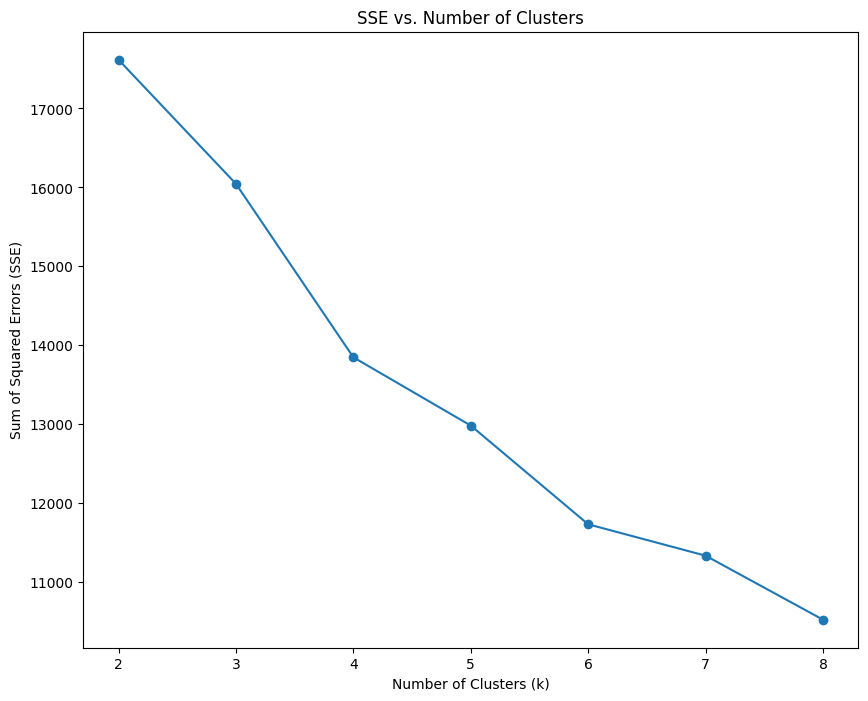
\includegraphics[width=0.8\linewidth]{img/sse-v-clusters.png}
        \caption{Sum of Squared errors vs Number of Clusters (k)}
        \label{fig:enter-label}
    \end{figure}

\item There should be 4 customer segments (clusters) based on the plot.
This is because of the slope in the inertia curve demonstrating an elbow (slope change) at
the third clustering solution (k = 4).

Inertia decreases as the number of clusters k increases because more clusters allow data points to be grouped closer to their respective centroids.
However, this trend weakens throughout the plot, the decrease in inertia becomes less significant, indicating diminishing returns with a larger number of smaller clusters, which might imply a loss in the generalization ability of that clustering solution, and be more computationally intensive.

\item K-modes would be a better clustering approach 
for this dataset. Out of the first 8 features, 6 are categorical 
variables (marital, education, default, housing, loan, contact)
and only 2 are numerical (age, balance). K-modes is generally
better at handling categorical data, while k-means is generally
better at handling numerical data. Additionally, One-Hot encoding
(done with \texttt{get\_dummies()}) is not necessary with k-modes.

K-modes uses a matching dissimilarity measure for categorical variables, which is more appropriate than the Euclidean distance used in k-means. This makes the clustering more meaningful for categorical data.
K-modes also represents cluster centers using modes rather than means, which makes more  sense for categorical data. 
\end{enumerate}

\vfill
\item StandardScaler
\begin{enumerate}
  \item Variability explained by top 2 components:

22.76\%
\vfill
\item We cannot clearly separate the three clusters, the inter-cluster distance is not considerable and there is a great deal of overlap between clusters so there is not a clear separation.
\begin{figure}[H]  % Forces the figure to stay here
  \centering
  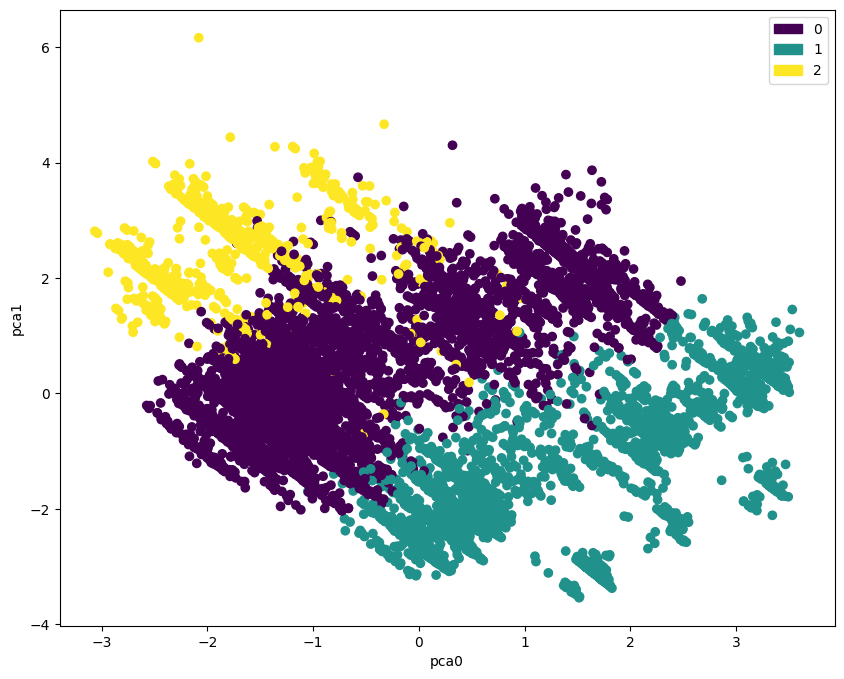
\includegraphics[width=0.8\linewidth]{img/pca-clusters.png}
  \caption{Scatter plot according to the first 2 PCs by cluster.}
\end{figure}
\newpage
\item The first thing that is more immediately clear is that the entirety of cluster
2 is comprised of \textit{retired} people, and all retired people belong to cluster 2,
and that cluster 2 observations have relatively lower education, being the one
with the greatest proportion of having only primary education and the one with
smallest proportion of tertiary and secondary education, which might suggest it's
an older population.
\begin{figure}[H]  % Forces the figure to stay here
  \centering
  \begin{subfigure}{0.49\linewidth}
      \centering
      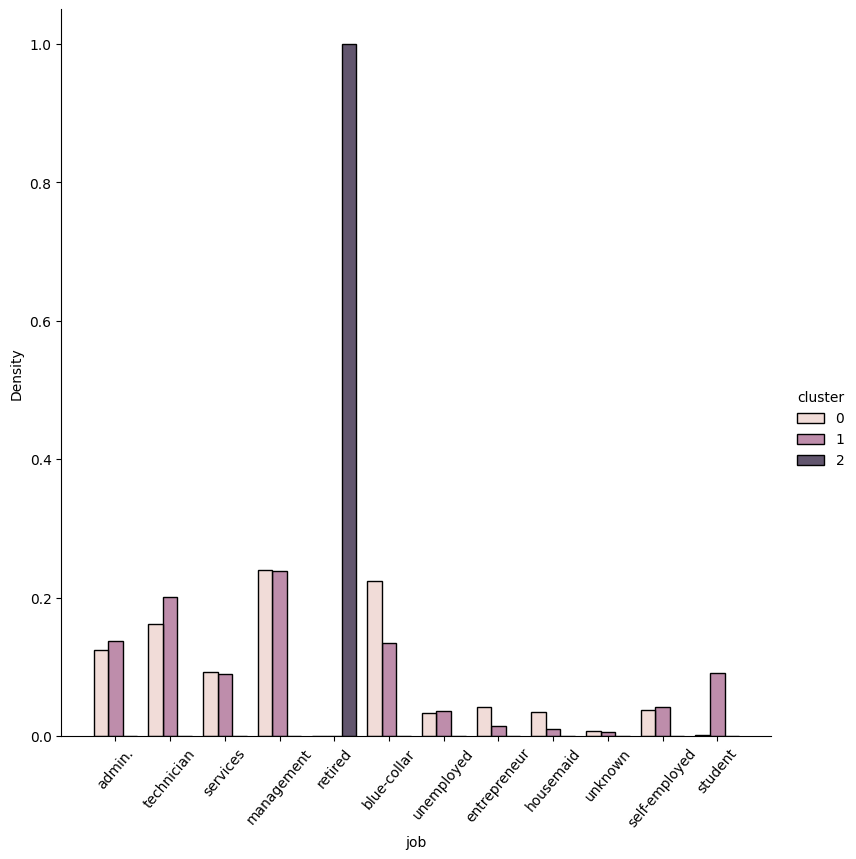
\includegraphics[width=\linewidth]{img/cluster-conditional-job-density.png}
      \caption{Cluster conditional job density distribution plot.}
  \end{subfigure}
  \begin{subfigure}{0.49\linewidth}
      \centering
      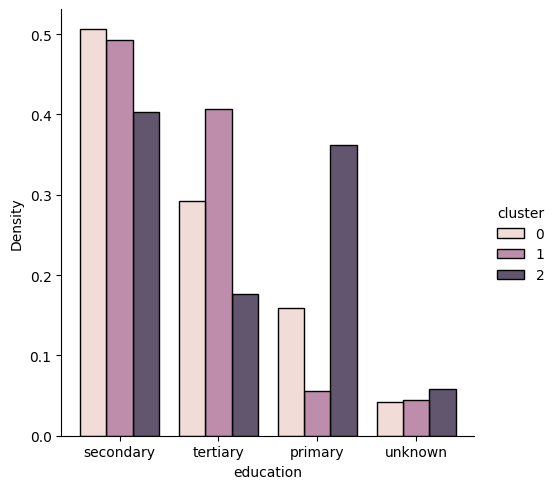
\includegraphics[width=\linewidth]{img/cluster-conditional-education-density.png}
      \caption{Cluster conditional education density distribution plot.}
  \end{subfigure}
\end{figure}

Cluster 0 and 1 are much more similar to each other with the notable
differences that regarding jobs, pratically every student belongs to cluster 1,
while cluster 0 has more blue-collar, entrepeneur and house-maid positions,
which might suggest that cluster 1 is generally younger. Also notable that cluster
1 has a proportionally higher level of education.

\end{enumerate}
\end{enumerate}

\newpage

% ----------------------------------------------------------------------
% Cover
% ----------------------------------------------------------------------

\end{document}

